\documentclass[12pt]{article}
%\usepackage[latin1]{inputenc}
\usepackage[T1]{fontenc}
\usepackage{geometry}
\usepackage{graphicx}
\usepackage{subcaption}
\usepackage[onehalfspacing]{setspace}
\usepackage{amsmath,amsfonts,amssymb,amsthm}
\usepackage{bm}
\usepackage{commath}
\usepackage{enumerate}
\usepackage{accents}
%\usepackage{enumitem}
\usepackage[shortlabels]{enumitem}
\usepackage{dsfont}
\usepackage{mathtools}
\usepackage{physics}
\usepackage{cite}
\usepackage[round]{natbib}
\usepackage{caption}
\captionsetup[figure]{font=small}
\usepackage{float}
\usepackage{hyperref}

\newtheorem*{theorem}{Theorem} 
\newtheorem*{lemma}{Lemma}
\newtheorem*{definition}{Definition}
\newtheorem*{corollary}{Corollary}
\newtheorem*{remark}{Remark}
\newtheorem*{example}{Example}
\newtheorem*{examples}{Examples}
\newcommand*{\QEDB}{\hfill\ensuremath{\square}}

\DeclareMathOperator*{\argmax}{arg\,max}
\DeclareMathOperator*{\argmin}{arg\,min}

\newcommand\independent{\protect\mathpalette{\protect\independenT}{\perp}}
\def\independenT#1#2{\mathrel{\rlap{$#1#2$}\mkern2mu{#1#2}}}

\interfootnotelinepenalty=10000
\allowdisplaybreaks
\geometry{
  left=2.5cm,
  right=2.5cm,
  top=2cm,
  bottom=2cm,
}

\graphicspath{{C:/Users/Simon/OneDrive/Uni/LMU/SS 2020/Statistisches Consulting/Bundestag-MP-Analyse/plots/}}

\begin{document}

\section{Results}

\subsection{Topical Content}

The STM provides an additional way to integrate covariate effects into the model, apart from prevalence variables that impact topic proportions across documents. To be specific, a categorical variable can be selected as topical content variable. While the prevalence variables influence the propensity of the 15 topics for each document, the content variable now allows for the word distributions for a given topic to vary across documents, according to content variable levels. Note that this is a completely new model, which is why one should not expect the resulting topics to be similar. 

Formally, recall that the word distribution used to eventually pick a word is $\beta_{d,n} := \beta(z_{d,n}, Y_d) \in \mathbb{R}^V$, where $z_{d,n}$ is a (latent) indicator variable determining the word's topic assignation and $Y_{d}$ is the document-level topical content variable with $A$ levels. In the prevalence model, no (document-level) topical content variable is specified, implying $\beta_{d,n} = \beta(z_{d,n})$; since $z_{d,n}$ is a word-level variable, $\beta_{d,n}$ is constant across all documents for a given topic $k$. When specifying a content variable $Y$, however, $\beta_{d,n}$ now varies for each document, according to the level $a \in \{1, ..., A\}$ the content variable takes on for document $d$. That is, the total number of $\beta$-vectors, each one of length $V$, now increases from $K$ to $K \times A$.

For our specific case, since the topical content variable needs to be categorical, we choose the variable \textit{party}, being categorical by definition and as it  is arguably the most significant factor in determining topic prevalence. IN doing so, we additionally posit that for a given topic, an MP's party also influences the vocabulary used when tweeting about that specific topic. For instance, this implies that an AfD party member tweets about immigration issues in a different linguistic manner than, say, a green MP. Since for the 2017 election period the German parliament contains members of 6 parties, $\bf{Y}$ is now a matrix with 10998 rows and 6 columns, yielding a total of 90 $\beta$-vectors.

After fitting the model, we proceed as for the prevelance model, that is, by inspecting top words and identifying topic labels. An additional difficulty, however, is that we do not have clear-cut top words per topic anymore; instead, we now have topic-level top words for each of the 15 topics, party-level top words for each of the 6 parties, as well as interaction top words for each of the 90 topic-party combinations. The table below presents topic labels for all 15 topics, identified by using the same 3-step procedure as for the prevalence model before. As can be seen, five topics are labeled as \textit{miscellaneous}, reflecting the complexity caused by the large number of $\beta$-vectors.

\begin{table}[h!]
	\centering
	\captionsetup{justification=centering,margin=2cm}
	\begin{tabular}{|l|l|}
	\hline
	Topic1  & Right/Nationalist 1  \\ \hline
	Topic2  & Miscellaneous 1      \\ \hline
	Topic3  & Left/Humanitarian    \\ \hline
	Topic4  & Housing       	   \\ \hline
	Topic5  & Innovation           \\ \hline
	Topic6  & Green/Energy         \\ \hline
	Topic7  & Miscellaneous 2      \\ \hline
	Topic8  & Corona               \\ \hline
	Topic9  & Foreign Affairs      \\ \hline
	Topic10 & Election             \\ \hline
	Topic11 & Right/Nationalist 2  \\ \hline
	Topic12 & Miscellaneous 3      \\ \hline
	Topic13 & Miscellaneous 4      \\ \hline
	Topic14 & Twitter/Politics     \\ \hline
	Topic15 & Miscellaneous 5      \\ \hline
	\end{tabular}
	\caption{List of topic labels for STM with topical content variable (party).}
	\label{Tab:labels_content}
\end{table}

The topical content model allows for vocabulary usage to differ across political parties, given a topic. In the graph below, we visualize this effect for the Corona topic, contrasting the green party "Bündnis 90/Die Grünen" with the right-wing nationalist party "AfD". The result is very insightful: even for a topic as clear-cut and novel as COVID-19, stark differences in terms of vocabulary usage arise. In particular, the AfD uses language suitable to describe immigration (\textit{migration}, \textit{grenz}) in order to discuss Corona, which very much reflects the unimodality of the party's political orientation. The green party, on the other hand, seems to address the topic much more specifically, mentioning key words like \textit{massnahm} or \textit{kind}.

\begin{figure}[h!]
  \centering
  \captionsetup{justification=centering,margin=2cm}
  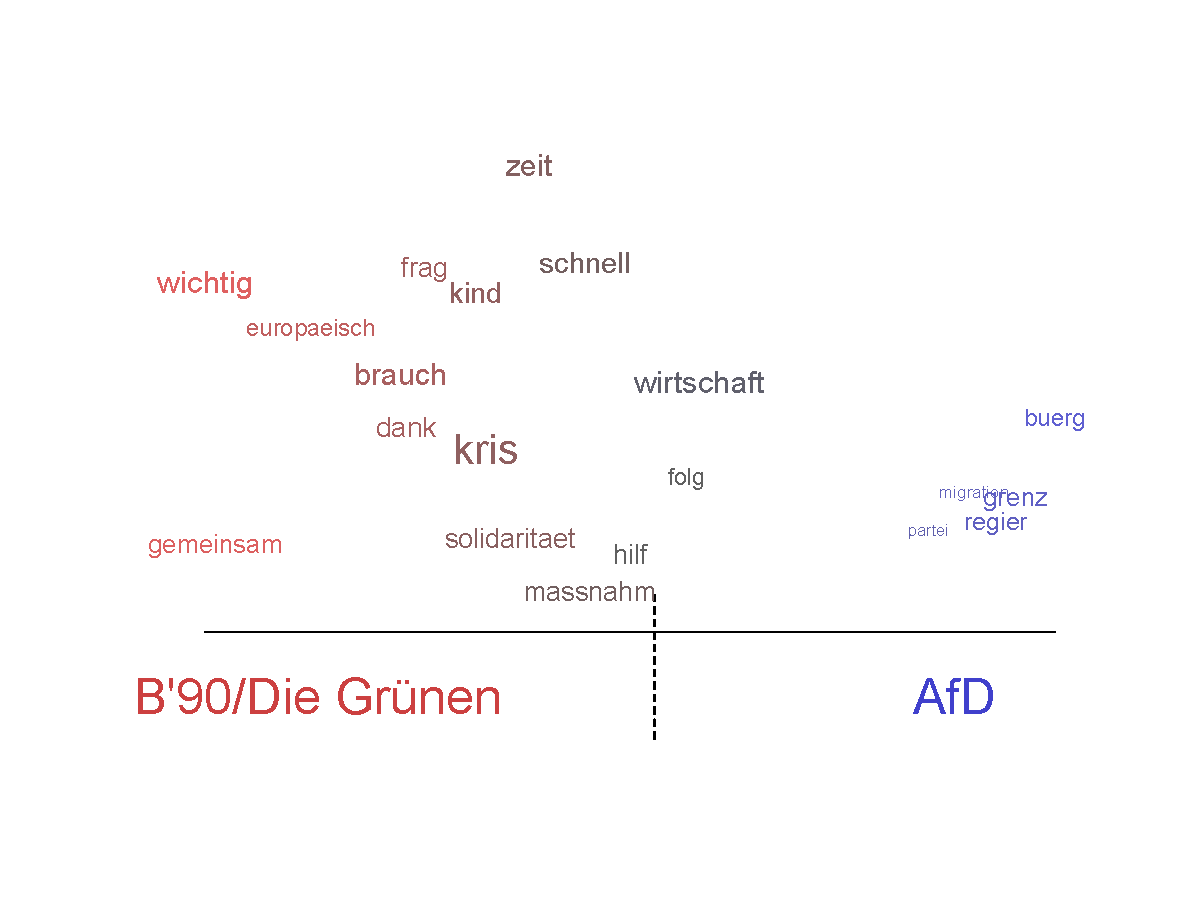
\includegraphics[scale = 0.5]{4_5/t8_vocab_parties.pdf}
  \caption{Differences in vocabulary usage across parties for the Corona topic.}
  \label{fig:t8_vocab_parties}
\end{figure}

While this type of visualization is indeed insightful, several concerns regarding the topical content model prevail: first of all, there is no natural candidate for the content variable, which - for labelling and interpretational purposes - should ideally be binary. Our dataset contains very few categorical variables, none of them binary. Furthermore, there is no natural, non-arbitrary way to binarize any of the covariates; for instance, binarizing the variable party, say, into conservative and liberal would misclassify at least one party. Therefore, our choice to use party as content variable is the result of a lack of alternatives, rather than being based on sound statistical or theoretical considerations. This, in turn, is reflected in the difficult labelling; for instance, one
third of all topics were eventually being labelled as miscellaneous. And while the previous illustration of inter-party differences in vocabulary usage is indeed insightful in terms of topic exploration and visualization, the aforementioned doubts lead us to discard the topical content variable for further analysis. In fact, in the next section we consider a model without any covariates in order to perform a clean 2-step procedure for covariate effect estimation.


\bibliography{bibliography}
\bibliographystyle{plainnat}

\end{document}